% This work is licensed under the Creative Commons Attribution 4.0 International License. To view a copy of this license, visit http://creativecommons.org/licenses/by/4.0/ or send a letter to Creative Commons, PO Box 1866, Mountain View, CA 94042, USA.

\documentclass[12pt, twoside]{report}
% Use package to keep preamble setup
\usepackage{manual}

\begin{document}
\title{Complexes Manual}
\titlepage
\date{2018}
\tableofcontents


\chapter{Introduction}
The complexes model is a hierarchical \gls{cg} protein model that has been
implemented with a Monte-Carlo engine to generate structures of protein
complexes \cite{Kim2008}. The model is commonly refereed to as the \gls{KH}
model in the literature. Since the original publication, the forcefield has been
used in a large variety of applications. Those include the study the binding
kinetics of the HIV-1 capsid proteins \cite{Zhu2015, Sha2017}, the kinetic
behavior of proteins in crowded environments \cite{Kim2013, Kim2010a, Rosen2011,
  Dignon2018a}, folding of knotted protein \cite{Skrbic2012, ABeccara2013,
  Sirur2013, Covino2014a, Sirur2016, Covino2013}, enhancing the structural
resolution of experiments \cite{Rozycki2011, Kofinger2015, Baumlova2014,
  Rozycki2015, Chalupska2017}, protein-protein interactions \cite{Okazaki2012,
  Malinverni2017, Ravikumar2012}, protein design \cite{Yadahalli2014}, docking
\cite{Fortoul2015}, multi-enzyme complexes \cite{Rozycki2017, N2018, Horan2018,
  Rozycki2016}. The model has also been extended to simulate intrinsically
disordered proteins and protein phase separation \cite{Dignon2018a}.

The complexes model is implemented in a \mbox{C++14} program \complexes and a
\mbox{Python} tool \pycomplexes. \complexes implements the Monte-Carlo engine
and \pycomplexes is a helper library and \gls{CLI} tool to setup simulations and
visualize them, see \cref{fig:toc}. The Monte-Carlo integrator accepts input
files in the \cplx format and configuration files for simulations. The split
enforces that a well defined file format exists that uniquely defines a
simulation. We have decided to use the YAML standard \cite{YAML} for the \cplx
files. A library to write YAML files exists for many programming languages
allowing easier integration into existing workflow without forcing a specific
programming language.

\begin{figure}[!ht] \centering
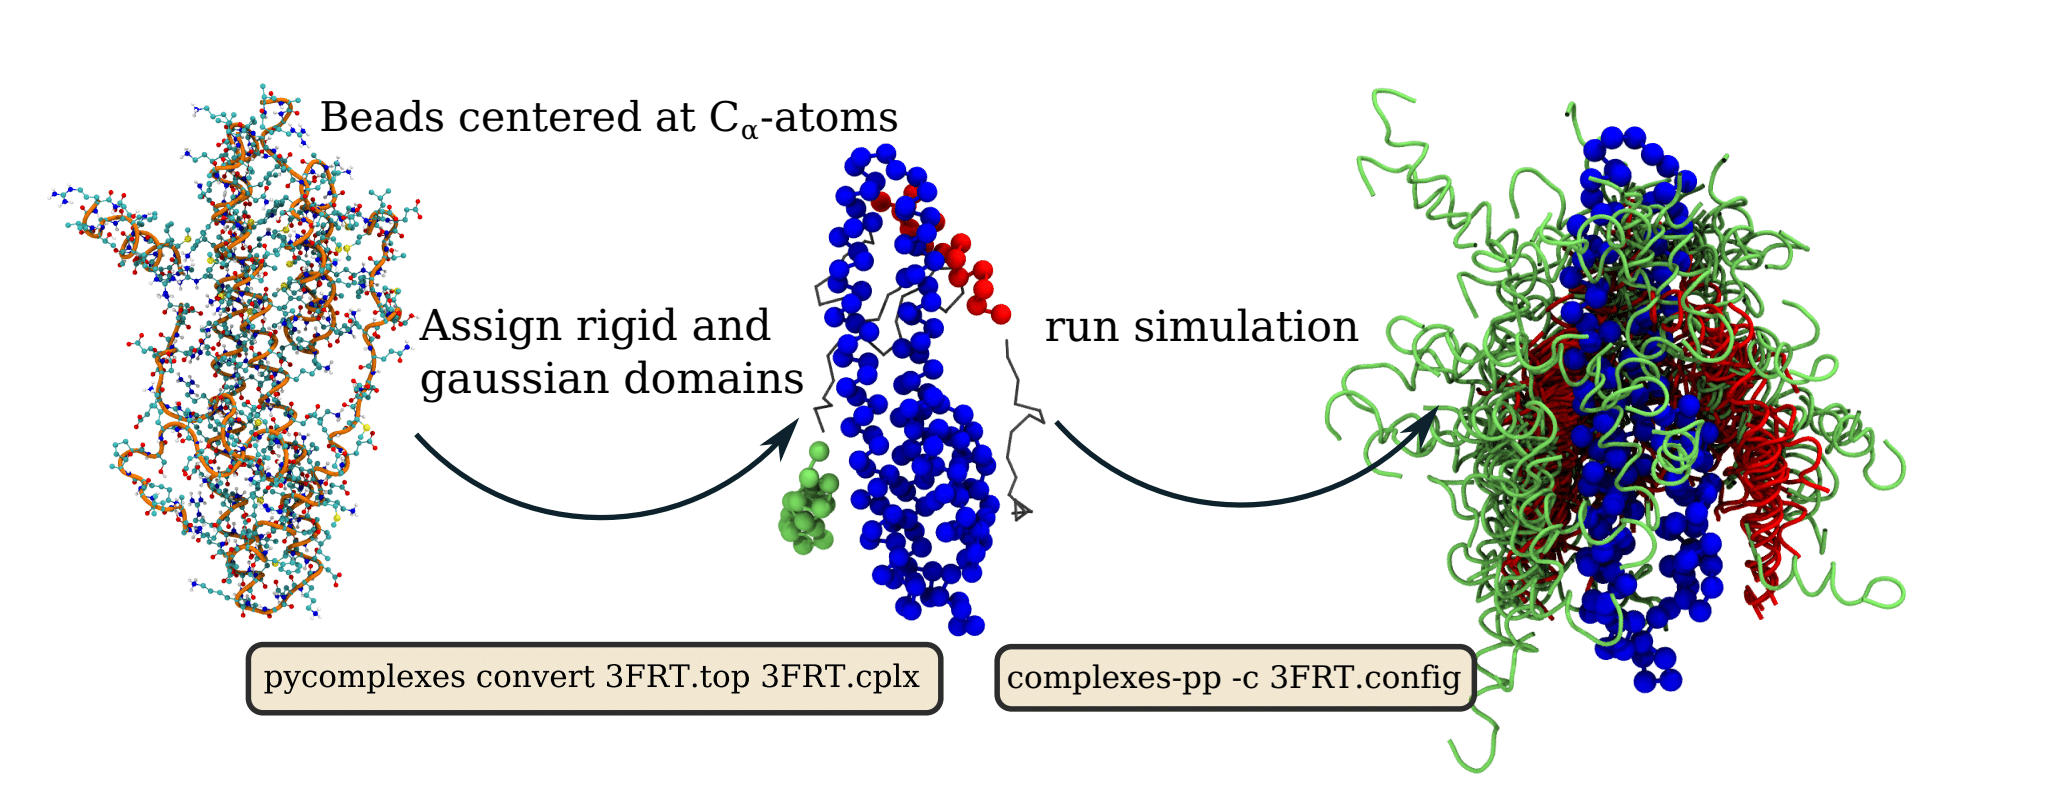
\includegraphics[width=\textwidth]{figures/toc}
\caption[\complexes use-case example.]{Example use case how to go from a single
known structure to an ensemble of structures using complexes. To prepare the
simulation domain types have to be assigned to amino acids and a \cplx file has
to be generated.}
\label{fig:toc}
\end{figure}

\chapter{Theory}

The complexes model describes proteins and large macromolecular structures at
three levels of coarse-graining. The first level is a bead. Beads are
interaction sites that are used to evaluate potentials and represent a single
amino acid, centered on the \calpha atoms. The second level is a domain. Domains
are collections of beads that define how the bead positions are propagated in a
simulation. The complexes model has rigid and flexible domains. The last level
is called a topology. It is a collection of connected domains. Topologies are
useful to develop efficient sampling algorithms for simulations with multiple
complexes. In this thesis, the general expression of the forcefield will be
referred to as the complexes model, when specific values for forcefield
parameters are given we refer to them as the \gls{KH} model. In the following,
the bead model and pair potential for different beads and different domains will
be explained.

\section{Beads}
\begin{figure}[!ht] \centering
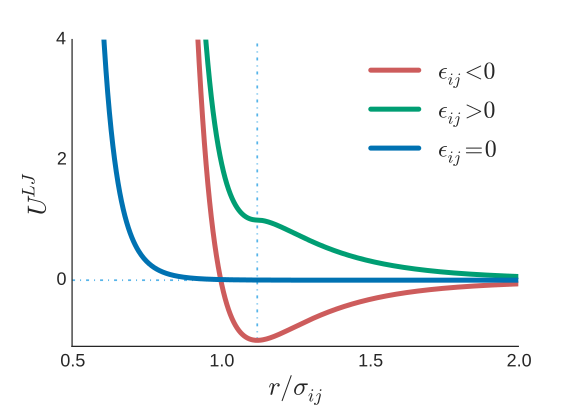
\includegraphics{figures/lennard-jones.pdf}
\caption[Modified Lennard Jones potential used in \complexes.]{Modified Lennard
Jones potential, \cref{eq:ch5:complexesLJ}, used in the complexes model in
reduced units. The attractive branch \(\epsilon_{ij}<0\) is shown in blue, the
repulsive part \(\epsilon_{ij}>0\) is shown in orange and the branch for
\(\epsilon_{ij}=0\) in green. The gray dashed line shows the minima at
\(2^{1/6}\) of the attractive branch.}
\label{fig:lennard-jones}
\end{figure} Beads are the interaction sites at which the force field and
additional restraint potentials are evaluated. In the complexes model
\cite{Kim2008} amino acids are modeled as single beads centered on the \calpha
atoms. As energy function, a Lennard-Jones like potential is used for effective
interactions of native and non-native contacts and a Coulomb term with an
exponential screening term for the electrostatics. The potential energies are by
convention calculated in units of \(\kT\), with \(T=\SI{300}{K}\) as the
reference temperature.

The Lennard-Jones like potential \(U_{LJ}\), between beads \(i\) and \(j\),
consists of four different branches to model attractive and repulsive
interactions
\begin{align}
  \label{eq:ch5:complexesLJ}
  U_{LJ} (r, \sigma_{ij}, \epsilon_{ij}) = \begin{cases}
    4 \epsilon_{ij} \left[\left(\frac{\sigma_{ij}}{r}\right)^{12} - \left(\frac{\sigma_{ij}}{r}\right)^{6}\right] &\mbox{if } \epsilon_{ij} < 0 \\
    4 \epsilon_{ij} \left[\left(\frac{\sigma_{ij}}{r}\right)^{12} - \left(\frac{\sigma_{ij}}{r}\right)^{6}\right] + 2 \epsilon_{ij} &\mbox{if } \epsilon_{ij} > 0 \mbox{ and } r < 2^{1/6} \sigma_{ij} \\
    - 4 \epsilon_{ij} \left[\left(\frac{\sigma_{ij}}{r}\right)^{12} - \left(\frac{\sigma_{ij}}{r}\right)^{6}\right] &\mbox{if } \epsilon_{ij} > 0 \mbox{ and } r > 2^{1/6} \sigma_{ij} \\
    .01 \left(\frac{\sigma_{ij}}{r}\right)^{12} &\mbox{if } \epsilon_{ij} = 0,
  \end{cases}
\end{align}
with $r$ the distance between the beads, the bead type pair parameters
\(\sigma_{ij}\) and \(\epsilon_{ij}\) for the contact distance and interaction
energy, respectively. For \(\epsilon_{ij} < 0\) this is the standard
Lennard-Jones potential, see \cref{fig:lennard-jones}. For \(\epsilon_{ij} > 0\)
this potential is purely repulsive, see \cref{fig:lennard-jones}. In case of
\(\epsilon_{ij}=0\) the potential is a hard wall slightly shorter than the
Lennard-Jones minimum of \(2^{1/6} \sigma_{ij}\) to avoid overlaps if additional
potentials are attractive and have singularities at \(r=0\), for example
electrostatic potentials. At contact \(r=\sigma_{ij}\) this potential gives
equal contributions from attractive and repulsive pairs with opposite sign. The
parameters \(\epsilon_{ij}\) are derived from the knowledge-based statistical
contact potentials \(e_{ij}\) by \gls{MJ} \cite{Miyazawa1996}. The \gls{MJ}
contact potentials have to be scaled to account for the added electrostatic
interactions and the preference of residue-residue to residue-solvent
interactions has to be balanced. In the complexes model this is done by scaling
with a parameter \(\lambda\) for the electrostatic interaction and shifting the
interaction with a parameter \(e_0\) for the residue-residue to residue-solvent
interactions with
\begin{align}
  \label{eq:ch5:complexesEpsilon} \epsilon_{ij} = \lambda (e_{ij} - e_0).
\end{align}
For the \gls{KH} model the values \(\lambda=0.159\) and \(e_0=\SI{-2.27}{\kT}\)
have been used, based on parametrizations to reproduce the experimental
determined second virial coefficient of hen egg lysozyme and the dissociation
constant \(K_d\) of the ubiquitin uim1 system \cite{Kim2008}. The contact
distances \(\sigma_{ij}\) are determined as weighted average \(\sigma_{ij} =
(\sigma_i + \sigma_j) / 2\) from the individual amino acids diameters,
\cref{tab:radii}. Note that in the original paper these values have been
incorrectly labeled as radii.
\begin{table}[!htb]
  \centering
  \begin{tabular}{c c c c c c c c c c}
    Ala&Arg&Asn&Asp&Cys&Gln&Glu&Gly&His&Ile \\
    \hline
    5.0&6.6&5.7&5.6&5.5&6.0&5.9&4.5&6.1&6.2 \\
    \\
    Leu&Lys&Met&Phe&Pro&Ser&Thr&Trp&Tyr&Val \\
    \hline
    6.2&6.4&6.2&6.4&5.6&5.2&5.6&6.8&6.5&5.9
  \end{tabular}
  \caption{Van-der-Waals diameters of amino acids in
    \AA\cite{Kim2008}.\label{tab:radii}}
\end{table}

The electrostatic potential consists of Coulomb interactions with an
ionic-screening term
\begin{align}
  \label{eq:ch5:complexesDH}
  U_{el}(r) = \underbrace{\frac{q_i q_j e^2}{4 \pi \epsilon_0 D_{el} r}}_{\text{coulomb}} \underbrace{\exp\left(\frac{-r}{\xi}\right)}_{\text{ionic-screening}} \underbrace{\frac{1}{\kT},}_{\text{scaling factor}}
\end{align}
with $e$ the elementary charge, $\epsilon_0$ the vacuum permittivity, $D_{el}$
the dielectric constant and \(\xi\) the Debye-length. The scaling factor of
\(1/\kT\) is used to convert the electrostatic energy into units of \(\kT\).
Bead charges are set according to amino acid type corresponding to a pH of 7.
Arginine and lysine are charged with $+e$, histidine with $+\frac{1}{2}e$, due
to its isoelectric point and aspartate and glutamine with $-e$. Charges for
other amino acids are set to 0. The ionic-screening term is used to set the salt
concentration of the environment with the Debye-length
\begin{align}
  \xi = \sqrt{\frac{\epsilon_r \epsilon_0 \kT}{e^2 N_A 2 I}},
\end{align}
where \(\epsilon_r\) the absolute permittivity, and \(I\) the ionic strength.
For a typical salt concentration of \SI{100}{mM} NaCl \(\xi \) is about
\SI{10}{\angstrom}.


\section{Domains}
Proteins and multiprotein complexes consist of multiple units that are connected
together. The domains are the second abstraction level of the complexes model
that connect beads. This abstraction is based on the assumption that a protein
complex consists of different proteins that behave as single units for a short
time span. There can be parts that are rigid during the lifespan of the protein
complex and short stretches of unstructured peptide chains that serve to tether
together as stiff parts. Domains are used to model this varied behavior. To
model the two different behaviors the complexes model has rigid and flexible
domains.

\subsection{Rigid Domain}
Rigid domains are the simplest form of a domain and the most versatile at the
same time. As the name suggests in a rigid domain the internal coordinates of
the beads in the domain do not change over time. Rigid domains are so versatile
because they can be used to model very different things. The obvious cases are
rigid protein parts like an $\alpha$-helix or a $\beta$-sheet. While not
described in the original complexes model it is possible to describe a rigid
domain at an even coarser level by grouping together amino acids. Using such a
\gls{cg} description requires finding new forcefield parameters for the
interactions but this versatility makes it possible to set up simulations that
incorporate experimental data with an appropriate detailed given experimental
uncertainties and prior knowledge.

\subsection{Flexible Domain}
\label{sec:flexible-domain} A compelling feature of the original complexes
implementation \cite{Kim2008} was its explicit treatment of flexible chains in
protein complexes. These chains served as an anchor to link rigid domains
together. In the original paper \cite{Kim2008} a peptide chain model using bond,
angle and dihedral potentials similar to \gls{MD} forcefields \cite{Hornak2006}
has been used. The advantage of such a model is that amino acids are modeled
explicitly and can interact with the rigid domains. A drawback of using this
model with a Monte-Carlo scheme is that only small movements of the whole chain
can be made to have small energy differences and therefore good acceptance
probabilities. As a side effect of this, the chain diffuses slowly through
configuration space and the overall diffusion of attached rigid domains is
limited by the linker instead of the translation and rotation step-size chosen
for the rigid domains. While such an explicit model can work for smaller
complexes \cite{Rozycki2011} it would make simulations of larger complexes
\cite{Kofinger2015} difficult.

A linker model that has a limited influence on the diffusion of the rigid
domains would be better suited to quickly sample configuration space. It has
been shown that for a linker only the length is important and not the exact
dynamics \cite{Rozycki2017}. We use this to make the assumption that the linker
only has to hold two rigid domains together and has no other functional purpose
and replace the explicit peptide chain with a \gls{PMF} that only depends on the
distance between the two rigid domains and the number of amino acids in the
linker. This \gls{PMF} potential acts as a restraint potential ensuring that the
distance between two rigid domains is physically correct. Because no explicit
beads are involved the diffusion of the rigid domains is only influenced by the
selected translation and rotation step-size. We can use a Gaussian chain polymer
model to calculate a suitable \gls{PMF}. Gaussian chains are suitable models
previously used to explain \gls{FRET} experiments \cite{OBrien2009}.

In the Gaussian chain model the beads are point particles connected by harmonic
springs. The average distance \(b\) between two beads determines the spring
constant. For a three dimensional chain the distances $R_{ij} = |\vec{r}_j -
\vec{r}_i|$ between beads \(i\) and \(j\), irrespective of the direction, is
distributed according to \cite{yamakawa1971modern}
\begin{align}
\label{eq:ch5:gaussian} P(R_{ij}) = 4 \pi R_{ij}^2 \left(\frac{3}{2\pi \langle
R^2_{ij}\rangle}\right)^{3/2} \exp\left(-\frac{3R_{ij}^2}{2 \langle
R_{ij}^2\rangle}\right) , R_{ij} > 0,
\end{align} where \(\langle R^2_{ij}\rangle = b^2(j-i)\) is the mean squared
distances between beads \(i\) and \(j\). The factor \(4 \pi R_{ij}^2\) is the
volume element of a shell with width \(dR\) and radius \(R_{ij}\). The
end-to-end distance for a Gaussian chain with $N$ beads is
\begin{align}
\label{eq:ch5:end2end} \sqrt{\langle R^2_{1N}\rangle} = \sqrt{N}b.
\end{align} To construct a \gls{PMF} for the Gaussian chain model we look at the
exponential term in \cref{eq:ch5:gaussian}. It is a similar expression as for
the Boltzmann distribution for a harmonic oscillator
\begin{align}
  \label{eq:ch5:harmonic-oscillator} V(\vec{r}_i, \vec{r}_j) =
\frac{3}{2b^2}\frac{1}{(j-i)}(\vec{r}_i - \vec{r}_j)^2,
\end{align} with spring constant $3/(b^2(j-i))$. From this the potential of mean
force between the ends of a Gaussian chain of length $N$ follows as
\begin{align}
  \label{eq:ch5:PMF} PMF(\vec{r}_1, \vec{r}_N) = \frac{3}{2 b^2} \frac{1}{N-1}
(\vec{r}_1 - \vec{r}_N)^2.
\end{align} To compare the distribution of end-to-end distances obtained from
this \gls{PMF} we run a Monte-Carlo simulation using \cref{eq:ch5:PMF} for a
linker of length \(N=200\) and a bond length \(b=\SI{3.81}{\AA}\)
\cite{Best2005}, see \cref{fig:gauss-model}. The distribution of end-to-end
distances created using the PMF agrees well with the expected distribution of
the Gaussian polymer model. This \gls{PMF} has been previously used to model
proteins and \gls{RNA} \cite{Hyeon2008}.
\begin{figure}[!ht]
  \centering
\includegraphics{figures/gauss-model}
\caption[Cumulative distribution function and probability density function of
the end-to-end distance $R$ for a Gaussian chain.]{Cumulative distribution
  function (top) and probability density function (bottom) of the end-to-end
  distance $R$ for a Gaussian chain of length $N=200$ and bond length
  $b=\SI{3.81}{\AA}$. The distributions for the ideal Gaussian chain are shown
  in orange. Results from an ensemble of 1 million distances obtained from a
  Monte-Carlo simulation using the PMF \cref{eq:ch5:PMF} are shown in blue. The
  value of the mean end-to-end distance, \cref{eq:ch5:end2end}, is marked in
  green.}
\label{fig:gauss-model}
\end{figure}

The final \gls{PMF} that we use will be between two beads of the two connected
rigid domains. These two beads have to be added to the length \(N\) of the
linker. Therefore the final \gls{PMF} for a linker of length \(N\) is
\begin{align}
  \label{eq:ch5:PMF-complexes} PMF(\vec{r}_0, \vec{r}_{N+1}) = \frac{3}{2 b^2}
\frac{1}{N+1} (\vec{r}_0 - \vec{r}_{N+1})^2,
\end{align} with \(\vec{r}_0\) and \(\vec{r}_{N+1}\) being the two beads of the
rigid domains that are connected by the linker.

\subsection{Generating Explicit Beads for Linker Model}

While the PMF, \cref{eq:ch5:PMF}, restraint potential, without explicit modeling
of the linker beads, is good for fast exploration of phase space some
applications, like the comparison of simulations to \gls{SAXS} measurements
\cite{Kofinger2015, Rozycki2011}, require to have explicit beads for the linker
domains. We now describe an iterative algorithm to generate positions for the
linker beads given fixed positions for the first and last bead of the linker.
\begin{figure}[!ht]
  \centering
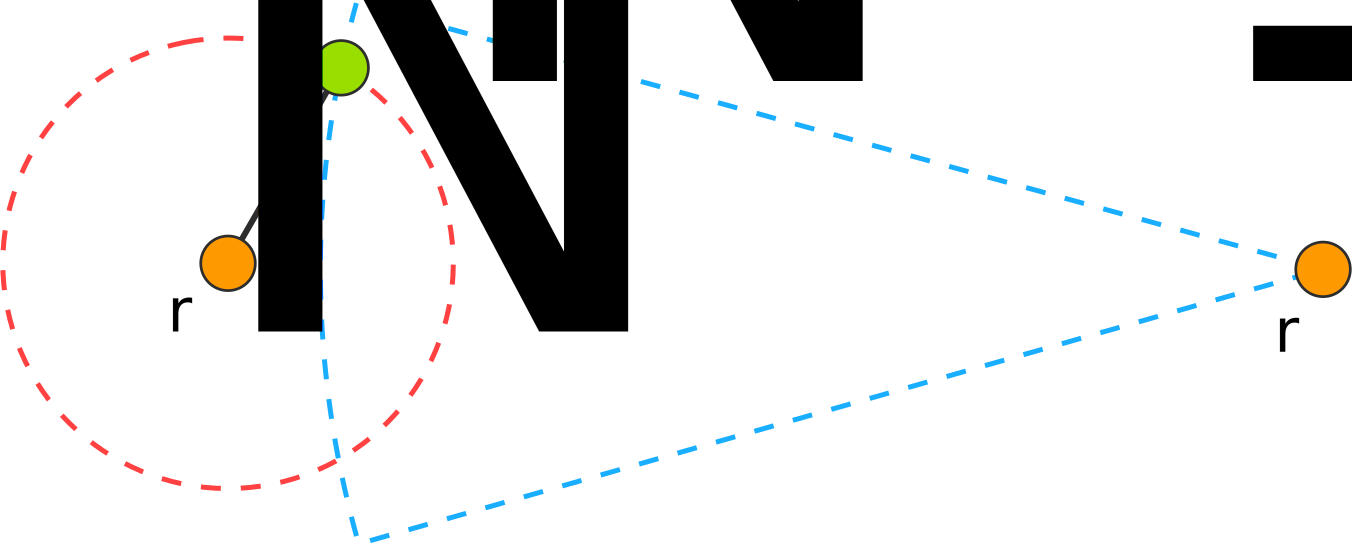
\includegraphics[width=\linewidth]{figures/gaussian_chain_move}
\caption[Illustration of generating bead distances for a Gaussian polymer
model.]{Example of distances drawn for a new bead $N-1$ (green) between to fixed
  endpoints (orange) of a Gaussian linker of length $N$ in two dimensions. The
  red circle is the distance between the beads $N$ and $N - 1$. This distance is
  randomly chosen from \cref{eq:ch5:gaussian}. The bead $N-1$ can be placed
  anywhere on this circle. The distance between bead $1$ and $N-1$ now has to be
  chosen so that circle (blue) drawn around bead $1$ intersects with the first
  circle (red). In two dimensions this restricts the positions of the new bead
  to the two intersection points. In three dimensions it would be restricted to
  a sphere. }
\label{fig:algorithm}
\end{figure} Given the positions of bead $N$ and $1$ a single bead $N-1$ can be
generated with the following algorithm:
\begin{enumerate}
\item Randomly choose a distance \(d_{\mathrm{start}}\) between bead $N$ and
$N-1$ distributed according to \cref{eq:ch5:gaussian}. This distance defines a
sphere around bead N on which bead \(N-1\) will be placed. (
\cref{fig:algorithm}, red circle)
\item Choose a distance \(d_{\mathrm{end}}\) between bead $1$ and $N-1$ so that
the sphere around bead $1$ intersects with the sphere calculated in step 1.
(\cref{fig:algorithm}, blue cone)
\item Choose a random point on the intersection of the red and blue sphere to
place the bead \(N-1\) (\cref{fig:algorithm}, green bead). In three dimensions
the intersection is a circle so a random angle $\theta$ has to be drawn.
\end{enumerate} To grow the next bead, with index $N-2$, simply repeat the
algorithm with bead $N-1$ as new starting point to choose the random distance
\(R_{N-1,N-2}\). Repeat this algorithm until all beads are generated.
\begin{figure}[!ht] \centering
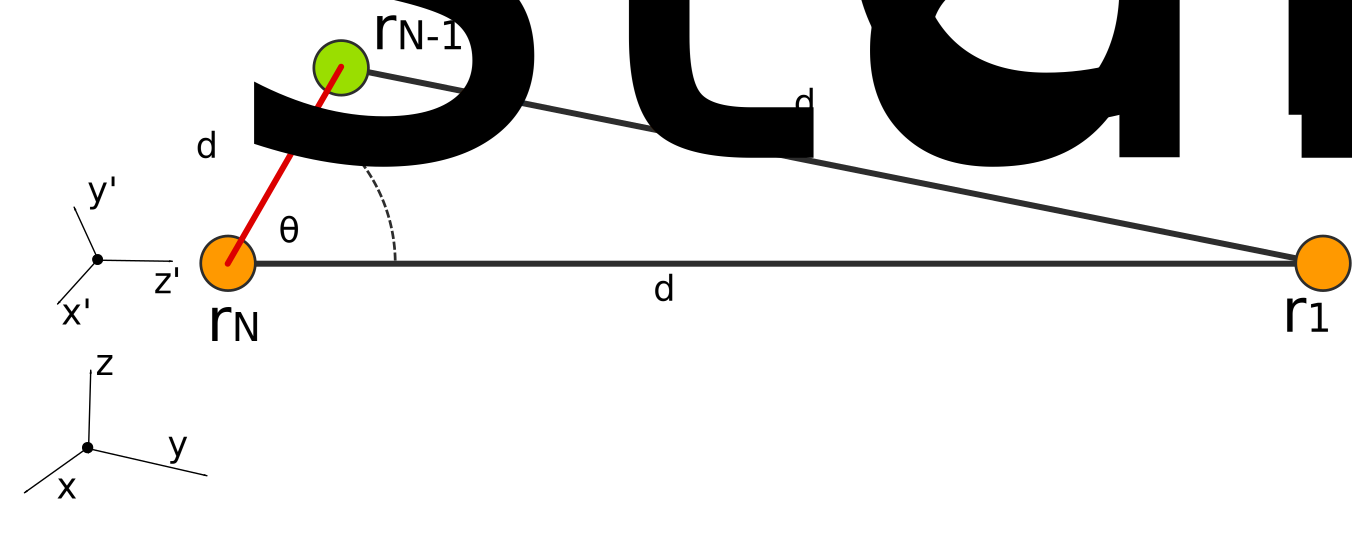
\includegraphics[width=\textwidth]{figures/gaussian_chain_bead_construction.pdf}
\caption[Illustration of generating bead positions for a Gaussian polymer
model.]{Schematic for calculating for calculating the position of bead
$\vec{r}_{N-1}$ given the positions of $\vec{r}_N$, $\vec{r}_1$, the distances
$d$, $d_{\mathrm{start}}$, $d_{\mathrm{end}}$ and an angle $\phi$ (not shown).
The coordinate system $(\vec{x}, \vec{y}, \vec{z})$ is our reference coordinate
system. The coordinate system $(\vec{x'}, \vec{y'}, \vec{z'})$ is used to
calculate $\vec{r}_{N-1}$.}
\label{fig:bead-construction}
\end{figure} This algorithm gives the three distance between the beads and
orientation that uniquely determines where a new bead should be placed. To
calculate the actual coordinates in the coordinate system of the simulation we
are using the following algorithm.
\begin{enumerate}
  \item Determine axis $\vec{z'}$ along the vector $\vec{r_N} - \vec{r_1}$.
  \item Determine perpendicular axes $\vec{x'}=\left(\frac{-z'_1-z'_2}{z'_0},1,
1\right)^T$ and normalize. Permutate in elements of $\vec{x'}$ if $z'_0=0$.
  \item Determine $\vec{y'} = \vec{x'} \times \vec{z'}$, with \(\times\) the
cross product.
  \item Determine angle \(\phi\) using the law of cosines
$\cos(\phi)=\frac{d_{\mathrm{start}}^2 + d^2 - d_{\mathrm{end}}^2}{ 2
d_{\mathrm{start}} d}$, with $d=|\vec{r_n} - \vec{r_1}|$ see
\cref{fig:bead-construction}.
  \item Calculate $\vec{r_{N-1}}$ in the coordinate system spanned by
$(\vec{x'}, \vec{y'}, \vec{z'})$ from the spherical coordinates given by
$(d_{\mathrm{start}}, \theta, \phi)$, see \cref{fig:bead-construction}.
  \item Convert $\vec{r_{N-1}}$ into reference coordinate system $(\vec{x},
\vec{y}, \vec{z})$.
\end{enumerate} Linker configurations generated using the above two algorithms
will include overlaps between neighboring beads, see \cref{fig:configuration}.
To avoid overlaps and generate more extended configurations it's sufficient to
add overlap checks in step 1 and 3 in the first algorithm algorithm, i.e. when
two beads are to close to each other.
\begin{figure}[!ht] \centering
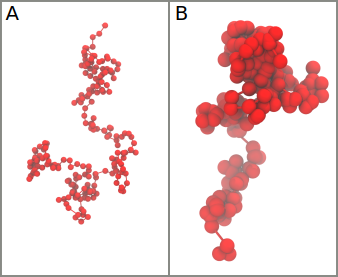
\includegraphics[width=.8\textwidth]{figures/configurations.pdf}
\caption[Example configuration generated for a Gaussian chain polymer model.]{
Gaussian chain with (left) and without (right) overlap check. Example
configuration for a alanine chain of length 200 with a bond-length of
$b=$\SI{3.81}{\AA}. All beads are drawn with a diameter of \SI{3.81}{\AA}.}
\label{fig:configuration}
\end{figure}

\subsection{Relaxation of Gaussian Polymerchain} The structures produced by
the Gaussian chain growing algorithms are not very physical. The distances
between beads vary by a standard deviation of \SI{1}{\AA} with a mean of
\SI{5}{\AA} in a single chain when the chain is grown with overlap checks. The
fluctuation in typical protein structures is less than a hundredth of an
\SI{}{\angstrom} with a mean distance of \SI{3.81}{\AA} \cite{Best2005}. For the
generation of more physical bead coordinates, it is, therefore, necessary to
relax the structures generated by the previous algorithm. For the relaxation,
the force field developed by \citet{Kim2008} can be used.

The forcefield consists of bond potentials for pseudobonds for
\(C_\alpha\!-\!C_\alpha\), angle potentials for pseudo angles
\(C_\alpha\!-\!C_\alpha\!-\!C_\alpha\) and torsion potentials for pseudo torsion
\(C_\alpha\!-\!C_\alpha\!-\!C_\alpha\!-\!C_\alpha\). The bond potential is a
harmonic potential
\begin{align} U_{\mathrm{bond}} = \frac{1}{2} k (r-r_0)^2,
\end{align} with \(r\) the \(C_\alpha\!-\!C_\alpha\) distance,
\(r_0=\SI{3.81}{\AA}\) the reference distance and \(k=\SI{378}{kcal ~ mol^{-1}
\AA^{-2}}\) the spring constant \cite{Karanicolas2002}. The pseudoangle
potentials is given a double well potential \cite{Best2005}
\begin{align} \exp[-\gamma U_{\mathrm{angle}}(\theta)] =
\exp[-\gamma(k_\alpha(\theta - \theta_\alpha)+\epsilon_\alpha)] + \exp[-\gamma
k_\beta(\theta - \theta_\beta)^2],
\end{align} where \(\theta\) is the angle between
\(C_\alpha\!-\!C_\alpha\!-\!C_\alpha\), the constants are
\(\gamma=\SI{0.1}{mol~kcal^{-1}}\), \(\epsilon_\alpha=\SI{4.3}{kcal ~
mol^{-1}}\), \(\theta_\alpha=\SI{1.6}{rad}\), \(\theta_\beta=\SI{2.27}{rad}\),
\(k_\alpha=\SI{106.4}{kcal ~ mol^{-1} rad^{-2}}\) and \(k_\beta=\SI{23.6}{kcal ~
mol^{-1} rad^{-2}}\). This potential accounts for the helical and extended
pseudoangles. The torsion potential is given by \cite{Karanicolas2002}
\begin{align} U_{\mathrm{torsion}}(\phi) = \sum_{n=1}^4 [1 + \cos(n\phi -
\delta_n)] V_n,
\end{align} where \(\phi\) is the torsion angle of the middle two beads in
\(C_\alpha\!-\!C_\alpha\!-\!C_\alpha\!-\!C_\alpha\). The constants \(V_n\) and
\(\delta_n\) are chosen for alanine as \(V_n=[0.936472, 2.307767, 0.131743
,0.613133]~\SI{}{k_{\mathrm{B}}T}\) and \(\delta_n=[287.354830,271.691192
,180.488748 ,108.041256]~\SI{}{rad}\) \cite{Karanicolas2002}.

The relaxation with the above described potential is done using a Monte-Carlo
algorithm. For trial moves the position of individual beads is changed. The
start and end bead are treated as fixed. For a linker of length \(N\) the
probability to pick a bead is uniform between all \(N-2\) beads that are allowed
to move. A sweep consists of \(N-2\) trial moves. Because the structure is only
supposed to be relaxed it isn't necessary to generate structures from an
equilibrium distribution and therefore detailed balance does not need to be
preserved. Here the move width is adjusted after each sweep to achieve a target
acceptance ratio of 30 \%. If after a sweep the acceptance ratio is larger than
30 \% the step-width is increased by 10 \% and decreased if the acceptance
ration is below 30 \%.

\begin{figure}[!ht] \centering
\includegraphics[width=.8\textwidth]{figures/linker-relaxation}
\caption[Monte-Carlo relaxation simulation of a Gaussian polymer
chain.]{Energies of a nonoverlapping Gaussian chain during relaxation. The chain
is 200 beads long and the initial structure was generated using the Gaussian
chain model with no overlaps. The acceptance rate during the Monte Carlo
simulation was set to target 30 \%. The bond energy is shown in blue, the angle
energy in orange, the torsion energy in green and the total energy in red.}
\label{fig:linker-relaxation}
\end{figure} Energy contributions for each potential from a relaxation run for a
chain of 200 beads is shown in \cref{fig:linker-relaxation}. In the beginning,
the energy is dominated by the bond potential, this is due to the fact that
average bond-length is larger than \SI{3.81}{\AA}. The bond lengths are fully
relaxed after around 200 sweeps. The angle potentials start to relax around
sweep 50 when the bond energy has already dropped by a factor of two. The angle
potential is fully relaxed after around 1000 sweeps. The last potential to relax
are the torsion angles. After about 500 sweeps the torsion angles start to see a
more pronounced decrease after 3000 sweeps when the other two potentials haven
been fully relaxed. The energy difference in the torsion potential from the
beginning of the simulation to the final structure is significantly less than
for the other two terms in the energy. The reason for this could be that the
starting structures generated by the Gaussian chain algorithm are particularly
ill chosen or that the simple spatial trial moves of the beads are not good for
relaxing this potential function.

\begin{figure}[!ht] \centering
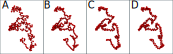
\includegraphics[width=.9\textwidth]{figures/linker-relaxation-comparison}
\caption[Gaussian polymer chain before and after relaxation with a physical
model.]{Linker configuration before relaxation (A) and after using only the bond
potential (B), using the bond and angle potential (C), and using the bond, angle
and torsion potential (D). All relaxation runs used the same initial structure
(A).}
\label{fig:linker-relaxation-comparison}
\end{figure} The structures generated by relaxing an initial configuration from
the Gaussian chain algorithm can be seen in
\cref{fig:linker-relaxation-comparison}. For comparison, single structures have
been generated with the full potential, only the bond potential, and the bond
and angle potential. The structures have all been generated from the same
initial structure and relaxation runs where 1000 sweeps long. The bond potential
alone has the biggest visual influence on the structure by achieving a more
uniform bond distance. The addition of the angle potential also gives a visual
improvement. Differentiating the bond and angle potential structure from the
structure with the full potential is difficult as both are very similar.

\subsection{Comparison of Unfolded Proteins and Linker Model} To understand
how well the model describes unfolded protein regions I will compare the radius
of gyration $R_G$, as a measure of compactness, of our model with experimental
data. For unfolded proteins the $R_G$ has been determined experimentally in
dependence on the protein length with denaturants \cite{Kohn2004}
\begin{align}
  \label{eq:ch5:plaxco} \langle R_G\rangle = R_0 N^{\nu},
\end{align} with \(R_0=1.927_{-0.238}^{+0.271}\)\SI{}{\AA} and \(\nu=0.598 \pm
0.028\). The radius of gyration of the Gaussian chain model is
\begin{align}
\label{eq:ch5:rg} \langle R_G\rangle = \sqrt{\frac{1}{6} \frac{N (N+2)}{N+1}} b
\approx \sqrt{\frac{1}{6}} N^{1/2} b.
\end{align} This scaling behavior is slightly different with \(\nu=.5\) and
\(R_0=\SI{1.555}{\AA}\). Therefore it is unlikely that the Gaussian polymer
without overlap checks reproduces the $R_G$ values of a denatured protein for
any number of beads.
\begin{figure}[!ht]
  \centering \includegraphics{figures/plaxco}
  \caption[Radius of gyration of Gaussian polymer chain for different chain
  lengths.]{Radius of Gyration computed for a linker with of different number of
    amino acids. For each length 1000 structures have been generated with
    overlap check (orange), without (blue), and fill relaxation (green). Error
    bars donate the standard deviation. The experimental $R_G$ scaling law for
    denatured proteins \cite{Kohn2004} is shown as gray line.}
\label{fig:plaxco}
\end{figure} To compare the \(R_G\) scaling behavior of the linker growth
algorithm to the scaling of denatured proteins we generate 1000 different
structures for a linker of 25 to 200 beads length. To get the values of a truly
free chain for each simulation the linker was padded with 25 beads in the front
and end so that only the middle $N$ beads have been used to calculate the $R_G$.
The bond-length was set to \SI{3.81}{\AA} \cite{Best2005}. Start and end points
have been placed at the optimal end-to-end distance, \cref{eq:ch5:end2end}.
Results are shown in \cref{fig:plaxco}. As anticipated without an overlap check
the $R_G$ values are systematically different. But with overlap checks enabled
the Gaussian polymer is within one standard of the experimental values if
$N<50$.

It should be noted that for intrinsically disordered proteins it has been shown
that the \(R_G\) with denaturants is larger than of the protein observed in
natural conditions \cite{Fuertes2017, Song2017, Zheng2016, Borgia2016}.
Therefore our Gaussian polymer model is a good enough description for the
flexible domains. A similar model has been employed to study intrinsically
disordered proteins \cite{Dignon2018a}.

\section{Topologies}

Topologies are a collection of connected domains. They can be used to model
large protein complexes that consist of multiple domains. The connection is
typically modeled as a distance based potential between two beads of the
connected domains. The connection potential can be chosen according to the
Gaussian chain model \cref{eq:ch5:PMF} or as a normal harmonic spring.

\chapter{Monte-Carlo Engine \complexes}

\complexes is a Monte Carlo simulation engine implementing the complexes protein
model. The program is written in modern \mbox{C++14} with a focus on being
extensible. The program contains an extensible Monte-Carlo engine, the modified
Lennard-Jones potential, \cref{eq:ch5:complexesLJ} and other pair potentials,
the Monte-Carlo movements for different domain types, and a cell-list algorithm
\cite{frenkel2001understanding} to speed up the energy evaluations.


\section{Flexible and Extensible Core Algorithms}

The core algorithms of the Monte-Carlo engine have the ability to add new trial
moves for domains and to add new Monte-Carlo algorithms for different
statistical ensembles or enhanced sampling techniques. This extensibility is
achieved thought a combination of run-time polymorphism and use of modern
\mbox{C++14}. In \complexes, this technique is used to implement domain trial
moves, Monte-Carlo algorithms, evaluation of pair potentials, and a cell-list
algorithm. In \mbox{C++} run-time polymorphism is implemented through abstract
classes and inheritance. In \complexes abstract classes are marked with the
preposition ``Abstract''. The most interesting abstract classes to add new
features to \complexes are \inlinecode{AbstractDomain},
\inlinecode{AbstractPairKernel}, \inlinecode{AbstractConnection},
\inlinecode{AbstractInteractionGrid} and \inlinecode{AbstractMcAlgo}. See
\cref{fig:Complexes} for a schematic how these classes interact with each other
during a simulation.
\begin{figure}[!ht] \centering
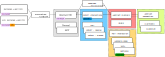
\includegraphics[width=\textwidth]{figures/software-model}
\caption[Complexes software overview.]{Schematic of the classes used in the
\complexes program and how they interact with each other (arrows). Abstract
classes and their explicit implementations are shown as colored boxes. Nested
boxes show different implementations of an abstract class. Names are as in the
code.}
\label{fig:Complexes}
\end{figure}

\section{Monte-Carlo Algorithm}

The main logic to run a Monte-Carlo simulation is implement in
\inlinecode{AbstractMcAlgo} with a virtual method called \inlinecode{sweep} to
implement a sweep. Currently \complexes implements sweep functions for the NVT
and N\(\Pi\)T ensemble \cite{frenkel2001understanding}. In addition two
different acceptance functions, Metropolis \cite{metropolis1953} and Glauber
\cite{Glauber1963} have been implemented as well. All Monte-Carlo sweep
algorithms work with all acceptance functions.

For a sweep in the NVT ensemble domains are chosen randomly from a uniform
distribution. If \(N\) is the number of domains that than a sweep will make
\(N\) trial moves and select a random domain with probability \(1/N\) for each
trial. In the N\(\Pi\)T ensemble trial moves are generated for the domains and
the volume. To account for the additional volume move a sweep consists of
\(N+1\) trial moves. At each trial, the probability to make a volume move is
\(1/(N+1)\). If a domain move was chosen the domain to be moved is chosen
randomly with a \(1/N\) probability. For the volume moves the domains are
re-scaled so that the centroid of the domain is scaled by
\(\sqrt[3]{(V+dV)/V}\). The N\(\Pi\)T algorithm is called NPT in the code and
configuration files.

\section{Boundary Conditions}

\complexes treats boundary effects using periodic boundary conditions
\cite{frenkel2001understanding}. Under these conditions, the centroid of all
domains is placed inside of the unit-cell. \complexes only implements
rectangular unit-cells. Because \complexes keeps the centroid of a domain within
the box it can happen that some beads are outside of the box.

To determine the distance between two beads \complexes uses the \gls{MIC}
\cite{frenkel2001understanding}. \complexes uses an efficient implementation to
calculate the minimum image distance, \cref{algo:fast-mic}. This algorithm is an
extension of a fast algorithm \cite{Deiters2013}, where the while-loop ensures
it works for any distance to ensure the algorithm will also work if trial moves
displace a domain by more than one periodic image. To ensure that the number of
iterations of the while-loop are as small as possible \complexes ensures that
the centroid of a domain are inside the unit-cell.
\begin{algorithm2e}[h!] \SetAlgoLined \DontPrintSemicolon \Fn{mic(distance[3],
box[3])} { \For{i=0; i<3; ++i}{ \While{distance[i] > .5 * box[i]} { distance[i]
-= box[i]\; } \While{distance[i] < .5 * box[i]} { distance[i] += box[i]\; } }
return distance; }
  \caption{Algorithm to efficiently convert the distance between two beads to
the minimum image distance it domain centers are inside of the simulation box.}
 \label{algo:fast-mic}
\end{algorithm2e}

\section{Replica Exchange Algorithms}

For enhanced sampling, \complexes implements replica exchange algorithms
\cite{Swendsen1986, Bennett1976, tuckerman2010statistical}. In replica exchange
simulations \(N\) independent copies of a simulation, which are further refereed
to as replicas, are run simultaneously and exchanged periodically. Implemented
are Temperature Replica Exchange \cite{Hansmann1997}, Hamiltonian replica
exchange \cite{Bussi2014} and pressure replica exchange \cite{Okabe2001}.

The implemented replica exchange algorithms differ by the acceptance function.
For temperature replica exchange the acceptance function for two configurations
\(i\) and \(j\) is \cite{Hansmann1997}
\begin{align}
  \label{eq:ch5:REMC} W(i\rightarrow j) = \min(1, \exp\left( (\beta_j - \beta_i)
(U(x_j) - U(x_i)) \right)),
\end{align} with $U$ being the energy function, \(x_i\) the configuration of
replica \(i\) and \(\beta_i\) the temperature of replica \(i\). For Hamiltonian
replica exchange the acceptance function is \cite{Bussi2014}
\begin{align}
  \label{eq:ch5:HREX} W(i\rightarrow j) = \min\left(1, \exp\left(
\frac{1}{\beta_i}(U_i(x_i) - U_i(x_j)) + \frac{1}{\beta_j}(U_j(x_j) - U_j(x_i))
\right)\right),
\end{align} with \(U_i\) the energy function of replica \(i\). For pressure
replica exchange the acceptance function is \cite{Okabe2001}
\begin{align}
  \label{eq:ch5:MPTMC} W(i\rightarrow j) = \min\left(1, \exp\left( (\beta_i -
\beta_j) (U(x_i) - U(x_j)) + (\beta_i P_i - \beta_j P_j) (V_i -
V_j)\right)\right),
\end{align} with \(P_i\) the pressure of replica \(i\) and \(V_i\) the volume of
replica \(i\).

The theoretical descriptions of the replica exchange algorithms do not specify
which replicas are exchanged in an attempt. To increase the probability to
accepted an exchange attempt in complexes only neighboring replicas are
exchanged \cite{Bussi2014}. During an exchange, not all neighboring pairs are
attempted to exchange, this is because the exchange between replica \(i\) and
\(i+1\) also depends on replica \(i-1\). Rather in \complexes attempts are only
done between even pairs when the attempt number is even and odd pairs otherwise.
In an even pair, of replicas \(i\) and \(i+1\), then \(i\) is even and odd for
odd pairs. For consistency 0 is counted as an even number and 1 as an odd
number.

Replica simulations require that multiple simulations are started. \complexes
requires that every replica is started in its own folder. Multiple simulations
can be started with the \inlinecode{--multidir} flag and a list of the folders
containing individual replicas. The \inlinecode{--multidir} option alone only
tells complexes to simulate multiple replicas to activate the exchange two flags
\inlinecode{--replex} and \inlinecode{--replex-accept} have to be used as well.
\inlinecode{--replex} states after how many sweeps an exchange should be
attempted. \inlinecode{--replex-accept} states the exchange function to be used.

The replica exchange simulations are also implemented in an extensible manner.
Because the different replicas exchange algorithms implemented require different
variables to be changed between the replicas, \complexes only exchanges the
coordinates of the beads and box dimensions during an exchange.


\section{Random Numbers}
\complexes uses pseudo random numbers to generate trial moves and accept moves.
As a pseudo \gls{RNG} it is using the mersenne twister \cite{Matsumoto1998}
implementation in the C++ standard library. Because the \gls{RNG} cannot be
safely used in a multi-threaded program like \complexes it uses a different
instance of the \gls{RNG} for each thread. The individual \gls{RNG} instances
are seeded from random numbers from an initial \gls{RNG} instance during setup.
To achieve reproducability \complexes requires the user to provide an explicit
seed for the initial \gls{RNG}. This requirement ensures that two runs with the
same input are identical on the same computation node.

\section{Pair Interactions Potentials}

In \complexes pair potentials are called pair kernels following a common
terminology used in computer science. The parameters of all available pair
kernels are given in the forcefield class. The parameters \(\sigma_{ij}\) and
\(\epsilon_{ij}\) are set according to bead type and shared between the
pair-kernels. During a simulation pair-kernels can be chosen for each individual
domain type pair present in the simulation, allowing to fine tune the
interactions. The Lennard-Jones like potential \cref{eq:ch5:complexesLJ} in
combination with the electrostatic potential \cref{eq:ch5:complexesDH}, and
several other potentials have been implemented. One additional potential is the
\gls{WCA} potential \cite{Weeks1971}
\begin{align}
  \label{eq:ch5:wca}
  U_{\mathrm{WCA}} (r, \sigma_{ij}, \epsilon_{ij}) = \begin{cases} -\epsilon_{ij} &\mbox{if } r < 2^{1/6}\sigma_{ij} \\
    4\epsilon_{ij} \left[ \left( \frac{\sigma_{ij}}{r} \right)^{12} - \left( \frac{\sigma_{ij}}{r} \right)^{6}\right] &\mbox{if } \epsilon_{ij} > 0.
  \end{cases}
\end{align}
An alternative version of the Lennard-Jones like potential that smoothly decays
to zero is implemented with the following smoothing term
\begin{align}
  \label{eq:ch5:smooth} F_{\mathrm{smooth}}(r, a, b) =
  \begin{cases} 1 &\mbox{if } r/\sigma_{ij} < a \\ 0 &\mbox{if } r/\sigma_{ij} >
b \\ \frac{(b^2 - (r/\sigma_{ij})^2 )^2 (b^2 + 2 (r/\sigma_{ij})^2 - 3 a^2)}{ (b
- a)^3} &\mbox{ otherwise },
  \end{cases}
\end{align}
with \(a=\SI{1.4}{\AA}\) and \(b=\SI{1.8}{\AA}\) being the bound in which the
potential decays to 0. The value for \(a\) and \(b\) are hard coded. A purely
repulsive potential with
\begin{align}
  U_{\mathrm{repulsive}} = \left( \frac{\sigma_{ij}}{r}\right)^{12}
\end{align}
is also implemented. Also implemented is a soft-core potential \cite{Antes2010a}
that allows to tune how soft the beads are and therefore they can potentially
overlap. The soft-core potential is a modification of the Lennard-Jones like
potential without the explicit repulsion branch,
\begin{align}
  U_{\mathrm{SC}}(r_{ij}) = 4\epsilon_{ij}\left[
\left(\frac{\sigma_{ij}^6}{\alpha\sigma_{ij}^6 + (r_{ij}-s)^6}\right)^2 -
\left(\frac{\sigma_{ij}^6}{\alpha\sigma_{ij}^6 + (r_{ij}-s)^6}\right)\right],
\end{align}
with \(\alpha\) the parameter to tune the softness of the beads, and
$s=\left(\sqrt[6]{2} - \sqrt[6]{2-\alpha}\right) \sigma_{ij}$ a shift parameter
to ensure that the minimum is always at \(\sqrt[6]{2}\) independent of
\(\alpha\). The other branches of the Lennard-Jones like potential can be
obtained by applying the same modifications. \(\alpha\) can be changed in the
range of zero to one, with \(\alpha=1\) allowing full overlap of the beads as
\(U_{\mathrm{SC}}(r=0)=0\) and \(\alpha=0\) recovering the Lennard-Jones like
potential \(U_{\mathrm{SC}}(r=0)=\infty\), \cref{eq:ch5:complexesLJ}. Because
this potential explicitly allows overlaps the electrostatics potential also has
to be changed to remove the divergence at \(r=0\). For this we use the potential
between two Gaussian charge distributions \cite{yarkony1995}
\begin{align}
  U_{\mathrm{el}}(r_{ij}) = \frac{q_i q_j}{4 \pi \epsilon_0
D}\frac{\mathrm{erf}\left(r_{ij}\sqrt{\lambda_{ij}}\right)}{r_{ij}}
\exp\left(-\frac{r_{ij}}{\zeta}\right) \frac{1}{\kT}
\end{align}
with \(\lambda_{ij}=\frac{\lambda_i \lambda_j}{\lambda_i + \lambda_j}\) and
\(\lambda_i\) the charge radius of bead \(i\). The charge radii are specified in
a forcefield for every bead type. In the standard \complexes forcefield all
radii are set to one.

The different pair kernels are implemented with a common abstract base class
\inlinecode{AbstractPairKernel}. The Lennard-Jones like and \gls{WCA} potential
have been implemented using Inastemp, a portable \gls{SIMD} library,
\cite{Bramas2017}.

\section{Bead and Domain Implementation}

No specific bead class exists in \complexes, instead, domains contain all
information specific to the beads as several lists. This design scheme follows
the ``struct of arrays'' pattern \cite{wikiAOS} used to optimize memory access.
For the beads a domain stores the coordinates in a \inlinecode{m\_xyz} field,
the charges in \inlinecode{m\_charges} and the bead types in
\inlinecode{m\_beads}. These three fields are the only information needed to
evaluate the potential energy with the pair potential functions. Domains are
also implemented with run-time polymorphism in an AbstractDomain class that
contains information about the beads and coordinates. Derived classes only need
to implement trial moves.

In addition to bead information, a domain also contains a unique id and a type
id that are defined at runtime. The type id is used to find the corresponding
pair kernel when evaluating the energy with a different domain. Choosing a
pair-kernel for domain type pairs and using a struct of arrays pattern allows
evaluating the pair-kernel for groups of beads. This pattern can be efficiently
implemented using inastemp \cite{Bramas2017}. Because the evaluation of the
pair-kernel is the most expensive calculation of \complexes this pattern ensures
that \complexes has good performance while using run-time polymorphism. The type
ids are also used to create domains with the same type of move but different
parametrizations for it. For example, the rigid domains have two parameters for
translation and rotation. Having the final parametrization set at runtime allows
creating two distinct rigid domain types for different proteins. This
flexibility is useful for simulations with a mixture of small and large domains.
The translation and rotation of larger domains can be chosen smaller to increase
the acceptance rate for their moves and small domains can be set to large
translation and rotation. Allowing to achieve optimal phase space exploration
rate for a simulation.

In \complexes only the rigid domain types is implemented. For the Monte-Carlo
moves the rigid domains can be translated by an arbitrary vector, each component
is chosen randomly from the range \([-a, +a]\), with \(a\) the maximal
displacement. The rotations are generated by choosing a random rotation axes in
the unit cube and a random rotation angle \cite{frenkel2001understanding}. This
method generates a known artifact that rotation axes along the edges are over
sampled. Because the all edges are equally sampled it does not affect generated
ensembles. In each trial move the probability to make a translation or a
rotation move is one half.

\section{Flexible Linkers and Connection Potentials}
As described in the theory flexible linker domains are replaced with effective
potentials from a Gaussian chain polymer model. For this \complexes implements
connection potentials in a \inlinecode{Connection} class. A connection contains
the ids of the two domains that are connected and the corresponding bead ids in
the domains. For each domain, a list of connections is stored in the class. So
if domains \(i\) and \(j\) are connected both contain the same connection. This
duplication of data makes it easier finding the corresponding connections for a
domain during the energy calculation. This compromise was chosen as it is
expected that the number of connections is significantly smaller the number of
beads. Currently implemented connection potentials are a flat potential (zero
everywhere), a harmonic potential, and a Gaussian chain \gls{PMF} potential,
\cref{eq:ch5:PMF-complexes}.

\section{Cell List Algorithm}

The other important part of the performance of complexes is the cell list
algorithm \cite{frenkel2001understanding} used to reduce the number of
interactions needed to evaluate. Cell-list algorithms reduce the computation
time to calculate the full energy from \(\mathcal{O}(N^2)\) to
\(\mathcal{O}(N)\) with \(N\) being the number of beads in a simulation. The
algorithm stores for every cell continues intervals of beads that are in the
corresponding cell. Every bead in a domain is given a unique id defined by the
order in which they appear in the input files. The interval will therefore only
store the id of the first bead entering the cell and the length of beads in the
cell. For domains that are larger than a single cell it can happen that two
different intervals are in a cell, see the red domain in
\cref{fig:celllist-datastructure} that has two intervals in the cell (1, 4). In
that case, the cell will store two intervals for the same domain. An intervals
is stored in the \inlinecode{CoInterval} class, \cref{listing:c++-celllist}.
Each cell stores a list of CoInterval instances. As an example of the data
stored for a list take the cell (1, 4) containing the red domain in
\cref{fig:celllist-datastructure}.
\begin{listing}[!ht]
  \begin{minted}{c++}
    class CoCell {
      // The list of intervals inside the current
      cell std::vector<CoInterval> m_intervals;
      // ...
    };

    class CoInterval {
      // The domain related to the current interval
      int m_domainId;
      // The position of the first element of the element-list
      int m_beginingOfInterval;
      // The number of elements in the current interval
      int m_nbElementsInInterval;
      // ...
    };
\end{minted}
\caption{Definition of the CoCell and CoInterval class used in the cell list
algorithm implemented in \complexes. The comment ``\inlinecode{...}'' indicates
other implementation details.}
\label{listing:c++-celllist}
\end{listing}
\begin{figure}[!ht] \centering
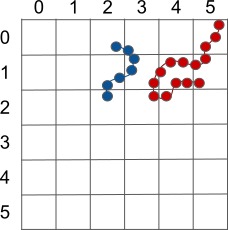
\includegraphics[]{figures/Complexesppintervals}
\caption[Cell list data-structure example.]{Example configuration for two
domains (blue and red) in a 2D grid. Numbers on the top and left are used to
index cells.}
\label{fig:celllist-datastructure}
\end{figure}

To calculate the completely potential energy between all domains we iterate over
all cells in the cell-list, see \cref{algo:cell-list}. For each cell we then
iterate over the list of CoIntervals.
\begin{algorithm2e}[h!] \SetAlgoLined \DontPrintSemicolon
  \Fn{computeEnergy(Cells[K], Domains[M])} { energy = 0\; \tcp{Compute energy
      (particle to particle interactions)} \For{cell \textbf{in} Cells}{
      \For{target \textbf{in} cell}{ \For{source \textbf{in} cell}{
          \If{source.domainId $\neq$ target.domainId}{ target\_dom =
            Domains[target.domainId]\; source\_dom = Domains[source.domainId]\;
            energy += kernel(target\_dom, source\_dom, target, source)\; } }
        \For{nb\_cell \textbf{in} cell.neighbors()}{ \For{source \textbf{in}
            nb\_cell}{ \If{source.domainId $\neq$ target.domainId}{ target\_dom
              = Domains[target.domainId]\; source\_dom =
              Domains[source.domainId]\; energy += kernel(target\_dom,
              source\_dom, target, source)\; } } } } } return energy }
 \caption{Cell list algorithm to calculate all pair interactions.}
 \label{algo:cell-list}
\end{algorithm2e}
During a Monte Carlo move only a single domain will be moved.
We therefore do not need to recalculate the complete potential energy. Instead
we need iterate over the cells occupied by the moved domain and update the
energy difference appropriately, replacing the outer most loop in
\cref{algo:cell-list} with a loop over only the cell currently occupied by the
domain. The last step further reduces the computational effort to calculate
energies during a simulation.

The interface to the cell list algorithm to calculate pair interactions has also
been implemented without references to the underlying algorithm and can be
swapped out with different algorithms. In \complexes, there are two
data-structures available for the cutoff grid. The \textit{dense} data structure
is allocated cell objects for all cells in a simulation box and offers efficient
computation of neighboring cells. The memory consumption of this data structure
scales with \((L_{\mathrm{Box}}/L_{\mathrm{Cell}})^3\), where
\(L_{\mathrm{Box}}\) is the edge-length of the simulation box and
\(L_{\mathrm{Cell}}\) is the edge-length of a cell, see
\cref{fig:container-memory-scaling}. This data structure is optimal for dense
simulations. The \textit{sparse} data structure uses a hash-map to only allocate
cells that are occupied by beads. The memory consumption of this data structure
scales with the number of beads in a simulation and is independent of the box
size. It is suited for sparse simulations. The high-level interface is also
agnostic to the underlying cell-list algorithm allowing to chose a completely
different algorithm if desired.
\begin{figure}[!ht]
  \centering
  \includegraphics{figures/container-memory-scaling}
  \caption{Memory consumption of the dense (blue) and sparse (orange) cell-list
    data-structure with a constant number of beads. The cutoff is set to
    \SI{12}{\AA}. The gray line marks one gigabyte.}
\label{fig:container-memory-scaling}
\end{figure}

\section{Task based parallelism}

Monte Carlo algorithms have two points which can be parallelized, the energy
calculation and the trial move generation. The trial move generation in
complexes is not computationally expensive and a minuscule amount of time is
spend on it. Leaving the energy calculation for the single replica simulations.
In replica exchange Monte-Carlo all replicas can be executed in parallel with
few synchronization points to exchange coordinates. Ideally, the single replica
and replica exchange simulation can use the same parallelisms scheme. It has to
be taken into account that replicas can be unbalanced or change during a
simulation if a phase transition occurs (from liquid to solid). Another
requirement was that it should be possible to always use the maximal number of
available \gls{CPU} cores independent of the number of replicas. Meaning a
single replica can use multiple threads and in the case that more replicas than
available threads are simulated the different replicas have a scheduler queue.

In \complexes this problem is solved using the task \gls{API} in OpenMP
\cite{openMP}. Tasks are generated based on either domains or cell lists (if
activate). Meaning tasks are small and plentiful. At the beginning of the energy
calculation, the number of tasks is distributed equally to the available
threads. If a thread finishes early it can then steal tasks from other threads.
Allowing threads to be always busy. It balances when different replicas have
different work loads. Nothing special is done to minimize the numa effect.
Therefore, it is maybe better to one process per memory node (explicit sync) and
threads inside.

The replica simulations can run in parallel. To make better use of available
resources that allow multi-node jobs also a \gls{MPI} implementation has been
developed. There is no work stealing between replicas in this configuration.

\section{\cplx File Format}

The input for \complexes simulation is stored in a \cplx file similar to the tpr
files in GROMACS. The \cplx file contains all information about the domains and
pair kernels to simulate, with the exception of the parameters for the
Monte-Carlo algorithm and the used forcefield parameters. The \cplx file format
is based on \yaml\cite{YAML} and divided into four sections \textit{box,
definitions}, \textit{topologies}, and \textit{forcefield}.

The \textit{box} section contains the dimensions of the rectangular simulation
box as a \yaml list. The length in each dimension is given in \SI{}{\AA}.

The \textit{definitions} section defines the type of domains that are used in
the simulation and the pair kernels used to calculate the energy between
domains. The \textit{definitions} section is separated into two sub sections to
define the final domain-types and their interactions between them, called
\textit{domains} and \textit{pair-interactions} respectively. The
\textit{domains} section contains a dictionary with the entry names being the
domain names and the definition for the domain. A definition contains the type
of move the domain can make, currently only rigid is implemented, and the parameters for
the move. Allowing to define several rigid bodies in a simulation that have
different rotation and translation parameters. The definitions can be used for
systems with a mixture of large and small rigid bodies to model the
corresponding mobility. The \textit{pair-interaction} section defines which pair
interaction potential to choose for each combination of domain types defined in
\textit{domains}. In the definition, one can define more domain types than what
will be used in a simulation. Allowing to create standard definitions (like the
\gls{KH} forcefield) for different applications. See
\cref{listing:cplx-definitions} for an example definition using two domain types
\textbf{A} and \textbf{EM}. Here the \textbf{EM} type is set to not move at all
and interacts with \textbf{A} domains using the \gls{WCA} potential. This
definition could be used to fit any domain of type \textbf{A} into a domain
defined by \textbf{EM}.
\begin{listing}[!ht]
  \begin{minted}{yaml}
    definitions:
      domains:
        A:
          defaults: {rotation: 2, translation: 1}
          move: rigid
       EM:
          defaults: {rotation: 0, translation: 0}
       move: rigid
    pair-interaction:
      - domain-type-pair: [A, EM] function: WCA
      - domain-type-pair: [A, A] function: LJH
      - domain-type-pair: [EM, EM] function: None
\end{minted}
\caption{\complexes domain definitions for a simulation with two domain types
\textbf{A} and \textbf{EM}. Both domain types move as rigid bodies but they have
different pair interaction potentials with each other.}
\label{listing:cplx-definitions}
\end{listing}

The \textit{topologies} section defines the actual domains that are used in the
simulation. It consists of a \yaml list of topology entries. Each topology entry
contains domain definitions and connections between domains of the same
topology. A domain contains the following field: beads, chain-ids, charges,
coordinates, nbeads, type, mc-moves, meta-data, name. Here the type field
specifies the domain type, which has to be defined in the definitions section.
Domains have to be numbered consecutively and uniquely across all topologies.

The \textit{forcefield} section contains definitions for the available bead
types as well as the energy and diameter pair parameters.

\chapter{pycomplexes toolbox}
\begin{listing}[!ht]
  \begin{minted}{yaml}
    box: [100, 100, 100]
    topology:
      protein-name:
        coordinate-file: structure.pdb
        move: true
        domains:
          A:
            type: rigid
            selection: 'namd CA and segid A'
          link:
            type: gaussian
            selection: 'name CA and segid L'
            start_connection: [A, 'segid A and resid 10']
            end_connection: [B, 'segid B and resid 10']
          B:
            type: rigid
            selection: 'name CA and segid B'
\end{minted}
\caption{TOP file for a simulation for two rigid domains connected by a Gaussian
domain. All selections are written in the atom selection language used by
MDAnalysis.}
\label{listing:top-definitions}
\end{listing} pycomplexes is a \mbox{Python} library and \gls{CLI} program that
includes several tools to help setup simulations for \complexes and analyze them
later. The \cplx format accepted by \complexes is very complex and allows the
user a lot of freedom in setting up the simulation. A lot of simulation setups
do not need to leverage the full flexibility of complexes and therefore
pycomplexes includes a tool called \inlinecode{convert} that takes as input a
simplified format, called a TOP file, for describing simulations and generating
\cplx files from it. As part of the conversion, the script will automatically
choose charges and interaction energies based on amino acid type. As interaction
energies, the user can choose either the \gls{KH} model or the unaltered
\gls{MJ} model. The charges are set according to the \gls{KH} model in both
cases. The interaction potential is chosen based on domain type, so far allowed
are rigid and gaussian. The rigid domain type uses the modified lennard jones
potential, \cref{eq:ch5:complexesLJ}. For the gaussian domains positions of the
\calpha beads will be stored in the \cplx as rigid domains that do not move and
a connection potential, \cref{eq:ch5:PMF}, will be used between the two rigid
domains connected by the gaussian domain. To define a domain in the top file the
type and a selection of beads have to be specified. For the gaussian domain, in
addition, the beads of the rigid domains connected by the gaussian domain have
to be specified as well. The convert script could ignore known beads for a
gaussian domain in the structure but keeping the information in the \cplx file
allows to generate explicit linker positions in the post processing, i.e. with
the \inlinecode{addlinker} tool.

The structures and selections are read and parsed using
MDAnalysis\cite{oliver_beckstein-proc-scipy-2016, Michaud-agrawal2011}. In the
molecular dynamics community there exists a large variety of structure file
format and they are often not well defined or popular programs write and accept
ill formatted files, MDAnalysis helps to read a large variety of different
formats with an easy to understand atom selection language.

In addition to the \inlinecode{convert} command pycomplexes also include a
variety of other commands to help the user setup and visualize simulations. As
of the time of writing the other implemented commands are
\begin{itemize}
  \item \inlinecode{equilibration} Update coordinates stored in a CPLX from a
trajectory.
  \item \inlinecode{forcefield} Convert a forcefield using scaling parameters
\(\lambda\) and \(e_0\), see \cref{eq:ch5:complexesEpsilon}.
  \item \inlinecode{visualize} Create VMD scripts from simulations.
  \item \inlinecode{demux} generate input files for the GROMACS tool
\inlinecode{trjcat} to generate time-continuous trajectories from replica
exchange simulations.
  \item \inlinecode{addlinker} generate explicit linker conformations for a
simulation with Gaussian linkers.
\end{itemize}



\clearpage
%%%%%%%%%%%%%%%%
% BIBLIOGRAPHY %
%%%%%%%%%%%%%%%%
\phantomsection
\addcontentsline{toc}{chapter}{Bibliography}
\bibliography{manual}
\clearpage
\printglossary[type=\acronymtype,title=List of Abbreviations]
\end{document}
